\documentclass[12pt]{article}
\usepackage[russian]{babel}
\usepackage{amsmath}
\usepackage{amsfonts,amssymb}
\usepackage{mathtools}
\usepackage{graphicx}
\usepackage{xcolor}
\selectcolormodel{gray}
\usepackage{subfig}
\textwidth 16.5cm \textheight 23cm \topmargin -1.5cm
\usepackage{algorithm}% http://ctan.org/pkg/algorithms
\captionsetup[algorithm]{labelformat=empty}
\usepackage[noend]{algpseudocode}
\usepackage{hyperref}

\newtheorem{theorem}{Теорема}
\newtheorem{lemma}{Лемма}
\newtheorem{corollary}{Следствие}
\newtheorem{definition}{Определение}
\newtheorem{remark}{Замечание}
\newtheorem{problem}{Задача}

\renewcommand{\div}{\mathop{\mathrm{div}}\nolimts}

\begin{document}
%\Large
    УДК 517.95
    \begin{center}
    {\bf ОПТИМИЗАЦИОННЫЙ МЕТОД ДЛЯ ЗАДАЧИ РАДИАЦИОННОГО ТЕПЛООБМЕНА С ГРАНИЧНЫМИ УСЛОВИЯМИ ТИПА КОШИ}
        \footnote[{1}]{$^)$Работа выполнена при финансовой поддержке РФФИ (проект 20-01-00113)}$^)$
    \end{center}
    \begin{center}
    {\bf \copyright\  2019 г.\ \  П.Р. Месенев, А.Ю. Чеботарев $^{*}$}
        \\
        {\it (690041 Владивосток,ул.Радио,7,ИПМ ДВО РАН)\\
        e-mail:  $^{*}$cheb@iam.dvo.ru}\\
        {\small  Поступила в редакцию 04.02.2020 г.\\
        Принята к публикации 2020 г.}
    \end{center}

    \sloppy
    \begin{quote}
        \small
        Исследована стационарная задача оптимального управления для уравнений
        радиационно-кондуктивного теплообмена в трехмерной области в рамках $P_1$--приближения уравнения
        переноса излучения.
        Показано, что последовательность решений экстремальных задач
        сходится к решению краевой задачи с условиями типа Коши для температуры.
        Результаты теоретического анализа проиллюстрированы численными примерами.
        Библ. 30.
    \end{quote}
    {\bf Ключевые слова:} уравнения радиационного теплообмена, диффузионное
    приближение, задача оптимального управления, условия типа Коши.

    \begin{center}
        \textbf{1. ВВЕДЕНИЕ. ПОСТАНОВКА ЗАДАЧИ ОПТИМАЛЬНОГО УПРАВЛЕНИЯ}
    \end{center}

    Стационарный радиационный и диффузионный теплообмен в
    ограниченной области $\Omega\subset \mathbb{R}^3$ с границей
    $\Gamma=\partial\Omega$ моделируется в рамках $P_1$--приближения для уравнения
    переноса излучения следующей краевой задачей~\cite{Modest,Kovt}:
    \begin{equation}
        \label{eq1}
        - a\Delta\theta + b\kappa_a(|\theta|\theta^3- \varphi)=0,\quad
        -\alpha \Delta \varphi + \kappa_a(\varphi-|\theta|\theta^3)=0,\; x\in\Omega.
    \end{equation}
    \begin{equation}
        \label{bc1}
        a(\partial_n\theta+\theta) = r,\;\;
        \alpha(\partial_n\varphi+\varphi) = u \text{  на  }\Gamma.
    \end{equation}
    Здесь $\theta$ -- нормализованная температура, $\varphi$ --
    нормализованная интенсивность излучения, усредненная по всем направлениям.
    Положительные физические параметры $a$, $b$, $\kappa_a$ и $\alpha$, описывающие
    свойства среды, определяются стандартным образом~\cite{Kovt}.
    Функция $r(x),\, x\in\Gamma$ является заданной, а неизвестная функция $u(x),\, x\in\Gamma$
    играет роль управления.
    Через $\partial_n$ обозначаем производную в направлении
    внешней нормали $\mathbf n$.

    Экстремальная задача заключается в отыскании тройки $\{\theta_\lambda,\varphi_\lambda,u_\lambda\}$
    такой, что
    \begin{equation}
        \label{cost}
        J_\lambda(\theta, u) = \frac{1}{2}\int\limits_\Gamma (\theta - \theta_b)^2d\Gamma +
        \frac{\lambda}{2}\int\limits_\Gamma u^2d\Gamma \rightarrow\inf
    \end{equation}
    на решениях краевой задачи (\ref{eq1}),(\ref{bc1}).
    Функция $\theta_b(x),\, x\in\Gamma$  и параметр регуляризации $\lambda>0$ заданы.

    Задача оптимального управления (\ref{eq1})--(\ref{cost}), если
    $r:=a(\theta_b+q_b)$, где $q_b$ -- заданная на $\Gamma$ функция,
    является при малых $\lambda$ аппроксимацией краевой задачи для уравнений (\ref{eq1}), в которой
    неизвестны краевые условия для интенсивности излучения $\varphi$, а ставятся
    граничные условия для температуры и тепловых потоков на границе,
    \begin{equation}
        \label{bc2}
        \theta|_\Gamma = \theta_b,\;\;
        \partial_n\theta|_\Gamma = q_b.
    \end{equation}


    В статьях~\cite{Pinnau07}--\cite{JMAA-19} представлен анализ
    краевых и обратных задач, а также задач управления
    для уравнений радиационного теплообмена
    в рамках $P_1$--приближения для уравнения
    переноса излучения.
    Различные краевые задачи, связанных с радиационным теплообменом
    изучены в~\cite{AmosA05}--\cite{Amosov18}.
    Нелокальная разрешимость
    нестационарной и стационарной краевых задач для уравнений сложного теплообмена
    без краевых условий на интенсивность излучения и
    с условиями (\ref{bc2}) для температуры доказана в~\cite{CNSNS19},\cite{CMMP20}.


    Основные результаты работы состоят в получении априорных оценок
    решения задачи (\ref{eq1}),(\ref{bc1}), на основе которых
    доказана разрешимость задачи оптимального управления
    (\ref{eq1})--(\ref{cost}) и выведена система оптимальности.
    Показано, что
    последовательность $\{\theta_\lambda,\varphi_\lambda,u_\lambda\}$ решений
    экстремальной задачи (\ref{eq1})--(\ref{cost}) при $\lambda\to +0$
    сходится к решению краевой задачи (\ref{eq1}),(\ref{bc2}) с условиями типа Коши для температуры.
    Результаты теоретического анализа проиллюстрированы численными примерами.


    \begin{center}
        \textbf{2. ФОРМАЛИЗАЦИЯ ЗАДАЧИ УПРАВЛЕНИЯ}
    \end{center}

    В дальнейшем считаем, что $\Omega\subset \mathbb{R}^3$~--- ограниченная строго липшицева
    область, граница $\Gamma$ которой состоит из конечного числа
    гладких кусков.
    Через $L^p$, $1 \leq p \leq \infty$ обозначаем
    пространство Лебега, а через $H^s$ -- пространство Соболева
    $W^s_2$.
    Пусть $H = L^2(\Omega), \; V = H^1(\Omega)$, через $V'$ обозначаем
    пространство, сопряженное с пространством $V$.
    Пространство $H$
    отождествляем с пространством $H'$, так что $V \subset H = H'
    \subset V'$.
    Обозначим через $\|\cdot\|$ стандартную норму
    в $H$, а через
    $(f,v)$ -- значение функционала $f\in V'$ на элементе $v\in V$,
    совпадающее со скалярным произведением в $H$, если $f\in H$.
    Через $U$ обозначаем пространство $L^2(\Gamma)$ с нормой
    $\|u\|_\Gamma=\left(\int_\Gamma u^2d\Gamma\right)^{1/2}.$



    Будем предполагать, что

    $(i) \;\; a,b,\alpha,\kappa_a, \lambda
    ={\rm Const}> 0 ,$

    $(ii) \;\, \theta_b, \,q_b \in U,\;\; r=a(\theta_b+q_b).$


    Определим операторы $A\colon V \to V'$, $B\colon U \to V'$, используя
    следующие равенства, справедливые для любых $y,z \in V$, $w\in U$:
    $$
    (Ay,z) = (\nabla y, \nabla z) +
    \int\limits_{\Gamma}yz d\Gamma, \;\;\; (Bw, z)
    = \int\limits_{\Gamma}wz d\Gamma.
    $$
    Билинейная форма $(Ay,z)$ определяет скалярное произведение
    в пространстве $V$, а соответствующая норма $\|z\|_V=\sqrt{(Az,z)}$ эквивалентна
    стандартной норме $V$.
    Поэтому определен непрерывный обратный оператор
    $A^{-1}:\,V'\mapsto V.$ Отметим справедливость, для любых
    $v\in V$, $w\in U$, $g\in V'$,
    следующих неравенств
    \begin{equation}
        \label{E}
        \|v\|^2\leq C_0\|v\|^2_V,\; \|v\|_{V'}\leq C_0\|v\|_V,\; \|Bw\|_{V'}\leq \|w\|_\Gamma,\;
        \|A^{-1}g\|_{V}\leq \|g\|_{V'}.
    \end{equation}
    Здесь постоянная $C_0>0$ зависит только от области $\Omega.$




    Далее используем следующее обозначение
    $[h]^s := |h|^s \mathrm{sign}\, h$,
    $s > 0$, $h \in \mathbb R$ для монотонной степенной функции.


        {\bf Определение.} Пара $\theta, \varphi\in V$
    называется {\it слабым решением} задачи (\ref{eq1}),(\ref{bc1}), если
    \begin{equation}
        \label{w1}
        a A \theta + b \kappa_a ([\theta]^4 - \varphi ) = Br,\quad
        \alpha A \varphi + \kappa_a (\varphi - [\theta]^4)  = Bu.
    \end{equation}

    Для формулировки задачи оптимального управления определим оператор
    ограничений $F(\theta, \varphi, u) : V \times V \times U \rightarrow V' \times V'$,
    \[
        F(\theta, \varphi, u) = \{ aA\theta + b \kappa_a ( [\theta]^4- \varphi) - Br,\;
        \alpha A \varphi + \kappa_a (\varphi -[\theta]^4) - Bu\}.
    \]


    \textbf{Задача $(CP)$.} Найти тройку $\{\theta, \varphi, u \} \in V \times V \times U$
    такую, что
    \begin{equation}
        \label{CP}
        J_\lambda(\theta, u) \equiv \frac{1}{2}\|\theta -\theta_b\|^2_\Gamma
        + \frac{\lambda}{2}\|u\|^2_\Gamma \rightarrow \text{inf},\;\; F(\theta, \varphi, u)=0.
    \end{equation}





    \begin{center}
        \textbf{3. РАЗРЕШИМОСТЬ ЗАДАЧИ $(CP)$}
    \end{center}

    Докажем предварительно однозначную разрешимость краевой задачи (\ref{eq1}),(\ref{bc1}).

    \textbf{Лемма 1.}
    {\it
    Пусть выполняются условия} (i),(ii), $u\in U$. {\it Тогда
    существует единственное слабое решение задачи (\ref{eq1}),(\ref{bc1}) и при этом}
    \begin{equation}
        \label{E1}
        \begin{aligned}
            a\|\theta\|_V \leq \|r\|_\Gamma + \frac{C_0\kappa_a}{\alpha}\|r+bu\|_\Gamma, \\
            \alpha b \|\varphi\|_V \leq \|r\|_\Gamma +
            \left(\frac{C_0\kappa_a}{\alpha} + 1\right)\|r+bu\|_\Gamma.
        \end{aligned}
    \end{equation}

    {\bf Доказательство.}
    Если второе уравнение в (\ref{w1}) умножить на $b$ и сложить с первым, то получим равенства
    \begin{gather*}
        A \left( a \theta + \alpha b \varphi \right) = B(r + bu),\;
        a\theta + \alpha b \varphi = A^{-1}B(r + bu),\;
        \varphi = \frac{1}{\alpha b}(A^{-1}B(r +bu) - a\theta).
    \end{gather*}
    Поэтому $\theta \in V$ является решением следующего уравнения:
    \begin{equation}
        \label{lemma-1-1}
        a A \theta + \frac{\kappa_a}{\alpha} \theta + b\kappa_a [\theta]^4 = g.
    \end{equation}
    Здесь $$g = Br + \frac{\kappa_a}{\alpha}A^{-1}B(r+bu) \in V'.$$
    Однозначная разрешимость уравнения~\eqref{lemma-1-1} с монотонной нелинейностью
    хорошо известна (см.
    например~\cite{Kufner}).
    Следовательно задача (\ref{w1})
    однозначно разрешима.

    Для получения оценок (\ref{E1}) умножим скалярно~\eqref{lemma-1-1} на $\theta \in V$ и отбросим неотрицательные
    слагаемые в левой части.
    Тогда
    $$
    a \|\theta\|^2_V \leq (g, \theta) \leq \|g\|_{V'}\|\theta\|_V,
    \quad a\|\theta\|_V \leq \|g\|_{V'}.
    $$
    Неравенства (\ref{E1}) позволяют оценить $\|g\|_{V'}$ и $\|\varphi\|_V $,
    $$
    \|g\|_{V'} \leq \|r\|_\Gamma + \frac{C_0\kappa_a}{\alpha}\|r + bu\|_\Gamma, \quad
    \|\varphi\|_V \leq \frac{1}{\alpha b} \|r + bu\|_\Gamma + \frac{a}{\alpha b} \|\theta\|_V.
    $$
    В результате получаем оценки~\eqref{E1}.

    \textbf{Теорема 1.}
    {\it
    Пусть выполняются условия} (i),(ii).
        {\it Тогда существует решение задачи $(CP).$
    }

        {\bf Доказательство.}
    Пусть $j_\lambda = \inf J_\lambda$ на множестве $u \in U$, $F(\theta, \varphi, u)=0.$
    Выберем минимизирующую последовательность
    $u_m \in U, \; \theta_m \in V$, $J_\lambda(\theta_m, u_m)
    \rightarrow j_\lambda,$
    \begin{equation}
        \label{MS}
        a A \theta_m +b \kappa_a([\theta]^4 - \varphi_m) = Br, \;\;
        \alpha A \varphi_m + \kappa_a (\varphi_m - [\theta]^4) = B u_m.
    \end{equation}
    Из ограниченности последовательности $u_m$ в пространстве $U$ следуют, на основании
    леммы 1, оценки
    $$
    \|\theta_m\|_V \leq C,\;\;
    \|\varphi\|_V \leq C,\;\;\|\theta_m\|_{L^6(\Omega)} \leq C.
    $$
    Здесь через $C>0$ обозначены различные постоянные, не зависящие от $m$.
    Переходя при необходимости к подпоследовательностям, заключаем, что
    существует тройка $\{ \hat{u}, \hat{\theta}, \hat{\varphi} \} \in U \times V \times V,$
    \begin{equation}
        \label{L}
        u_m \rightarrow \hat{u} \text{  слабо в } U, \;\;
        \theta_m, \varphi_m \rightarrow \hat{\theta}, \hat{\varphi} \text{
            слабо в } V, \text{
            сильно в } L^4(\Omega).
    \end{equation}
    Заметим также, что $\forall v \in V$
    \begin{equation}
        \label{L1}
        |( [\theta_m]^4 - [\hat{\theta}]^4, v) \leq
        \leq 2 \| \theta_m - \hat{\theta}\|_{L^4(\Omega)} \|v\|_{L^4(\Omega)}
        \left( \| \theta_m \|^3_{L_6(\Omega)} + \| \hat{\theta} \|^3_{L_6(\Omega)}\right).
    \end{equation}
    Результаты о сходимости~\eqref{L},\eqref{L1} позволяют перейти
    к пределу в~\eqref{MS}.
    Поэтому
    \[
        a A \hat{\theta} + b \kappa_a ([\hat{\theta}]^4 - \hat{\varphi} = Br), \;
        \alpha A \hat{\varphi} + \kappa_a (\hat{\varphi} -[\hat{\theta}]^4) = B \hat{u},
    \]
    и при этом $j_\lambda \leq J_\lambda(\hat{\theta}, \hat{u}) \leq \liminf J_\lambda(\theta_m, u_m) =
    j_\lambda$.
    Следовательно тройка $\{\hat{\theta}, \hat{\varphi}, \hat{u} \}$ есть
    решение задачи $(CP).$





    \begin{center}
        \textbf{4. УСЛОВИЯ ОПТИМАЛЬНОСТИ}
    \end{center}

    Для получения системы оптимальности достаточно использовать
    принцип Лагранжа для гладко-выпуклых экстремальных задач~\cite{10,11}.
    Проверим справедливость ключевого условия, что образ производной
    оператора ограничений $F(y, u)$, где $y=\{\theta,\varphi\}\in V\times V$,
    совпадает с пространством $V'\times V'.$ Именно это условие гарантирует
    невырожденность условий оптимальности.
    Напомним, что
    $$
    F(y, u) = \{ aA\theta + b \kappa_a ( [\theta]^4- \varphi) - Br,\;
    \alpha A \varphi + \kappa_a (\varphi -[\theta]^4) - Bu\}.$$


    \textbf{Лемма 2.}
    {\it
    Пусть выполняются условия} (i),(ii).
        {\it Для любой пары $\hat{y} \in V \times V, \hat{u} \in U$ справедливо равенство}
    \[
        \texttt{Im}F_y'(y, u) = V' \times V'.
    \]


        {\bf Доказательство.} Достаточно проверить, что задача
    $$
    aA \xi + b \kappa_a (4|\hat{\theta}|^3 \xi - \eta) = f_1, ;\ \;
    \alpha A \eta + \kappa_a (\eta - 4|\hat{\theta}|^3 \xi) = f_2
    $$
    разрешима для всех $f_{1,2}\in V'.$ Данная задача равносильна системе
    $$
    aA\xi + \kappa_a\left(4b|\theta|^3 + \frac{a}{\alpha}\right) \xi = f_1
    +\frac{\kappa_a}{\alpha}f_3, ;\ \;
    \eta =\frac{1}{\alpha b}( f_3-a\xi).
    $$
    Здесь $f_3=A^{-1}(f_1+bf_2)\in V.$ Разрешимость первого уравнения указанной системы очевидным образом следует из
    леммы Лакса-Мильграма.


    В соответствии с леммой 2, лагранжиан задачи $(CP)$ имеет вид
    $$
    L(\theta, \varphi, u, p_1, p_2) = J_\lambda(\theta, u)
    + (aA\theta + b\kappa_a([\theta]^4 - \varphi) - Br, p_1)
    + (\alpha A \varphi + \kappa_a(\varphi - [\theta]^4) - Bu, p_2).
    $$
    Здесь $p=\{p_1,p_2\}\in V\times V$ -- сопряженное состояние.
    Если $\{\hat{\theta}, \hat{\varphi}, \hat{u} \}$ -- решение задачи $(CP)$, то
    в силу принципа Лагранжа~\cite[Теорема 1.5]{10} справедливы вариационные равенства
    $\forall v\in V,\, w\in U$
    \begin{equation}
        \label{OC1}
        (\hat{\theta} -\theta_b, v)_\Gamma + (aAv + 4 b\kappa_a |\hat{\theta}|^3v, p_1)
        - \kappa_a ( 4 |\hat{\theta}|^3v, p_2) = 0,\;
        b \kappa_a (v, p_1)+ (\alpha A v + \kappa_a v, p_2) = 0,
    \end{equation}
    \begin{equation}
        \label{OC2}
        \lambda(\hat{u},w)_\Gamma - (Bw, p_2) = 0.
    \end{equation}
    Таким образом, из условий~\eqref{OC1},\eqref{OC2}
    получаем следующий результат

    \textbf{Теорема 2.}
    {\it
    Пусть выполняются условия} (i),(ii).
        {\it  Если $\{\hat{\theta}, \hat{\varphi}, \hat{u}\}$ -- решение
    задачи $(CP)$, то существует единственная пара $\{p_1, p_2 \} \in V\times V$
        такая, что}
    \begin{equation}
        \label{eq:as}
        aAp_1 +4|\hat{\theta}|^3 \kappa_a(bp_1 - p_2) = B(\theta_b - \hat{\theta}), \;\;
        \alpha A p_2 + \kappa_a (p_2 - b p_1)=0
    \end{equation}
    {\it и при этом} $\lambda\hat{u} = p_2.$




    \begin{center}
        \textbf{5. АППРОКСИМАЦИЯ ЗАДАЧИ С УСЛОВИЯМИ ТИПА КОШИ}
    \end{center}


    Рассмотрим краевую задачу для уравнений сложного теплообмена, в которой нет краевых условий на
    интенсивность излучения.
    \begin{equation}
        \label{eq11}  - a\Delta\theta + b\kappa_a([\theta]^4- \varphi)=0,\quad
        -\alpha \Delta \varphi +
        \kappa_a(\varphi-[\theta]^4)=0,\; x\in\Omega.
    \end{equation}
    \begin{equation}
        \label{bc11} \theta=\theta_b,\quad \partial_n\theta = q_b \text{  на  }\Gamma.
    \end{equation}
    Существование $\theta,\varphi\in H^2(\Omega)$, удовлетворяющих~\eqref{eq11},\eqref{bc11}
    для достаточно гладких
    $\theta_b,\, q_b$ и достаточные условия единственности решения
    установлены в~\cite{CMMP20}.
    Покажем, что решения задачи $(CP)$ при $\lambda\to+0$
    аппроксимируют решение задачи~\eqref{eq11},\eqref{bc11}.


    \textbf{Теорема 3.}
    {\it
    Пусть выполняются условия} (i),(ii) {\it и существует решение задачи~\eqref{eq11},\eqref{bc11}.}
        {\it  Если $\{\theta_\lambda,\varphi_\lambda,u_\lambda\}$ -- решение
    задачи $(CP)$ для $\lambda>0$, то существует последовательность
        $\lambda\to +0$
        такая, что}
    $$
    \theta_\lambda\rightarrow\theta_*, \;\; \varphi_\lambda\rightarrow\varphi_*
    \text{ слабо в }V,\text{ сильно в }H,
    $$
        {\it где $\theta_*,\varphi_*$ -- решение задачи~\eqref{eq11},\eqref{bc11}.}

        {\bf Доказательство.}
    Пусть $\theta,\varphi\in H^2(\Omega)$ -- решение задачи~\eqref{eq11},\eqref{bc11},
    $u=\alpha(\partial_n\varphi+\varphi)\in U.$ Тогда
    $$
    a A \theta + b \kappa_a ([\theta]^4 - \varphi ) = Br,\quad
    \alpha A \varphi + \kappa_a (\varphi - [\theta]^4)  = Bu,
    $$
    где $r:=a(\theta_b+q_b).$ Поэтому, с учетом того, что $\theta|_\Gamma=\theta_b$,
    $$
    J_\lambda(\theta_\lambda, u_\lambda) = \frac{1}{2}\|\theta_\lambda -\theta_b\|^2_\Gamma
    + \frac{\lambda}{2}\|u_\lambda\|^2_\Gamma\leq J_\lambda(\theta, u)=\frac{\lambda}{2}\|u\|^2_\Gamma.
    $$
    Следовательно,
    $$
    \|u_\lambda\|^2_\Gamma\leq C,\;\; \|\theta_\lambda -\theta_b\|^2_\Gamma\to 0,\; \lambda\to +0.
    $$
    Здесь и далее $C>0$ не зависит от $\lambda.$
    Из ограниченности последовательности $u_\lambda$ в пространстве $U$ следуют, на основании
    леммы 1, оценки
    $$
    \|\theta_\lambda\|_V \leq C,\;\;
    \|\varphi\|_\lambda \leq C.
    $$
    Поэтому можно выбрать последовательность $\lambda\to+0$ такую, что
    \begin{equation}
        \label{LL}
        u_\lambda \rightarrow u_* \text{  слабо в } U, \;\;
        \theta_\lambda, \varphi_\lambda \rightarrow \theta_*,\varphi_* \text{
            слабо в } V, \text{
            сильно в } L^4(\Omega).
    \end{equation}
    Результаты~\eqref{LL} позволяют перейти к пределу при $\lambda\to+0$
    в уравнениях для $\theta_\lambda,\varphi_\lambda,u_\lambda$ и тогда
    \begin{equation}
        \label{CC}
        a A \theta_* + b \kappa_a ([\theta_*]^4 - \varphi_* ) = Br,\quad
        \alpha A \varphi_* + \kappa_a (\varphi_* - [\theta_*]^4)  = Bu_*.
    \end{equation}
    При этом $\theta_*|_\Gamma=\theta_b.$
    Из первого уравнения в~\eqref{CC}, с учетом, что $r=a(\theta_b+q_b)$,
    выводим
    $$
    - a\Delta\theta_* + b\kappa_a([\theta_*]^4- \varphi_*)=0 \text{ п.в. в }\Omega,\quad \theta_*=\theta_b,\quad
    \partial_n\theta = q_b \text{ п.в. на  }\Gamma.
    $$
    Из второго уравнения в~\eqref{CC} следует, что $-\alpha \Delta \varphi +
    \kappa_a(\varphi-[\theta]^4)=0$ почти всюду в $\Omega.$ Таким образом,
    пара $\theta_*,\varphi_*$ -- решение задачи~\eqref{eq11},\eqref{bc11}.




    \begin{center}
        \textbf{6. ЧИСЛЕННЫЕ ЭКСПЕРИМЕНТЫ}
    \end{center}

    Представим итерационный алгоритм решения краевой задачи~\eqref{eq1}--\eqref{bc2} управления.
    Пусть $\tilde J_\lambda(u)=J_\lambda(\theta(u), u)$, где $\theta(u)$ компонента решения
    задачи~\eqref{eq1},\eqref{bc3}, соответствующая управлению $u\in U$.

    В соответствии с~\eqref{eq:as} градиент функционала $\tilde J_\lambda(u)$ равен
    \[
        \tilde J'_\lambda (u) = \lambda u - p_2.
    \]
    Здесь $p_2$ -- соответствующая компонента сопряженного состояния из системы~\eqref{eq:as},
    где $\hat{\theta}\coloneqq\theta(u)$.

    \begin{algorithm}[H]
        \caption{Алгоритм градиентного спуска}
        \label{alg:algorithm}
        \begin{algorithmic}[1]
            \State Выбираем значение градиентного шага $\varepsilon$,
            \State Выбираем количество итераций $N$,
            \State Выбираем начальное приближение для управления $u_0 \in U$,
            \For{$k \gets 0,1,2,\dots,N$}
                :
                \State Для данного $u_k$ рассчитываем состояние $y_k = \{\theta_k, \varphi_k\}$ --
                решение задачи~\eqref{eq1},\eqref{bc1}.
                \State Рассчитываем значение функционала качества $J_\lambda(\theta_k, u_k)$.
                \State Рассчитываем сопряженное состояние $p_k=\{p_{1k},p_{2k}\}$ из уравнений~\eqref{OC1},
                где $ \hat{\theta} \coloneqq \theta_k, \hat{u}=u_k$.
                \State Пересчитываем управление $u_{k+1} = u_k - \varepsilon (\lambda u_k - p_2)$
            \EndFor
        \end{algorithmic}
    \end{algorithm}
    Значение параметра $\varepsilon$ выбирается эмпирически таким образом, чтобы значение
    $\varepsilon (\lambda u_k - p_2)$ являлось существенной поправкой для $u_{k+1}$.
    Количество итераций $N$ выбирается достаточным для выполнения условия
    $J_\lambda(\theta_k, u_k) - J_\lambda(\theta_{k+1}, u_{k+1}) < \delta$, где $\delta>0$ определяет точность расчетов.

    Примеры, рассмотренные ниже, иллюстрируют работоспособность предложенного алгоритма при
    малых, что важно, значениях параметра регуляризации $\lambda \leq 10^{-12}.$
    В первом примере приводится сравнение расчетов по
    предложенному алгоритму с результатами работы~\cite{CNSNS19}.
    Во втором примере выполнены тестовые расчеты для куба.

    \textbf{Пример 1.}

    Приведем примеры расчетов для куба
    $\Omega = {(x, y, z), 0 \leq x,y,z \leq l}$.
    Будем считать, что $l=1~\text{см}$, $a = 0.006[\text{см}^2/\text{c}]$,
    $b=0.025[\text{см}/\text{с}]$,
    $\kappa_a=1[\text{см}^{-1}]$, $\alpha = 0.(3)[\text{см}]$.
    Указанные параметры соответствуют стеклу~\cite{Grenkin5}.
    Параметр регуляризации $\lambda=10^{-12}.$

    Пусть граничные данные $r$ и $u$ в~\eqref{bc3} имеют вид:
    \begin{gather*}
        r = 0.7,\quad
        u = \hat u = 0.5.
    \end{gather*}
    Далее рассчитываем состояние $\theta$ и $\varphi$ как решение задачи~\eqref{eq1},\eqref{bc3} и в качестве
    $\theta_b$ выбираем граничные значение функции $\theta$ на $\Gamma$.
    Значения нормальной производной $\partial_n\theta$ на $\Gamma$ должны соответствовать
    значениям $q_b=r/a-\theta_b.$
    Применяя предложенный алгоритм с начальным приближением $u_0 = 0.1$, находим приближенное решение
    $\{\theta_\lambda,\varphi_\lambda,u_\lambda\}$ задачи (CP)\@.
    Для демонстрации того, что алгоритм находит приближенное решение задачи с данными
    Коши для температуры, важно сравнить значения $\partial_n\theta_\lambda$ на $\Gamma$ с $q_b.$

    На рисунке~\ref{fig:img_test_11_iso} представлен модуль относительного отклонения $\partial_n\theta_\lambda$ от $q_b$
    на грани куба в плоскости $z=l$, где $\partial_n\theta_\lambda=\partial\theta_\lambda/\partial z$,
    а также динамика функционала качества, определяющего норму разности $\|\theta_\lambda -\theta_b\|^2_\Gamma$.
    На остальных гранях куба значения относительного отклонения имеют тот же порядок малости.
    \begin{figure}[H]
        \centering
        \subfloat[$|q_n - \partial_n\theta_\lambda|$]
        { \label{fig:img_test_11} 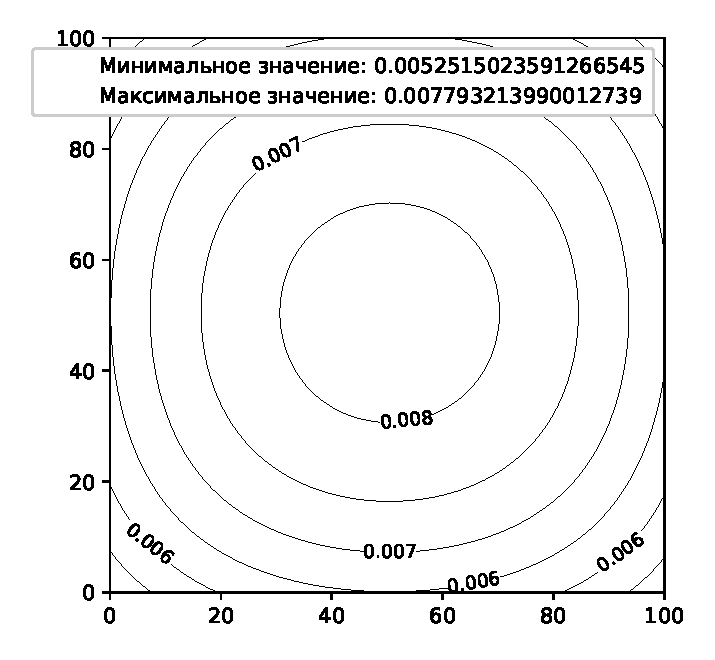
\includegraphics[width=.49\linewidth]{img/exp11/theta_n_diff_iso}
        }
        \subfloat[Изменение функционала в зависимости от числа итераций]
        { \includegraphics[width=.49\linewidth]{img/exp11/quality} }
        \caption{Результаты первого эксперимента}
    \end{figure}
    \begin{figure}[H]
        \centering
        \subfloat[$|q_n - \partial_n\theta_\lambda|$]
        { \label{fig:img_test_11_cube} 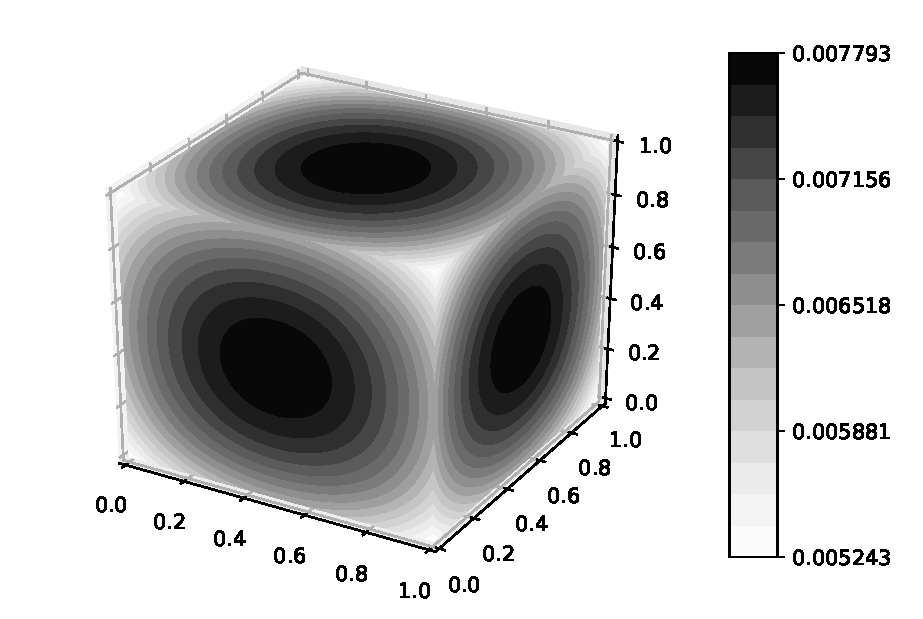
\includegraphics[width=.49\linewidth]{img/exp11/theta_n_diff_cube}
        }
        \subfloat[Изменение функционала в зависимости от числа итераций]
        { \includegraphics[width=.49\linewidth]{img/exp11/quality} }
        \caption{Результаты первого эксперимента}
    \end{figure}

    \textbf{Пример 1. С константными граничными условиями}

    Приведем примеры расчетов для куба
    $\Omega = {(x, y, z), 0 \leq x,y,z \leq l}$.
    Будем считать, что $l=1~\text{см}$, $a = 0.006[\text{см}^2/\text{c}]$,
    $b=0.025[\text{см}/\text{с}]$,
    $\kappa_a=1[\text{см}^{-1}]$, $\alpha = 0.(3)[\text{см}]$.
    Указанные параметры соответствуют стеклу~\cite{Grenkin5}.
    Параметр регуляризации $\lambda=10^{-12}.$

    Пусть граничные данные $r$ и $u$ в~\eqref{bc3} имеют вид:
    \begin{gather*}
        r = 0.8 cos(\frac{\pi}{2}x) + 0.1,\quad
        u = \hat u = 0.5.
    \end{gather*}
    Далее рассчитываем состояние $\theta$ и $\varphi$ как решение задачи~\eqref{eq1},\eqref{bc3} и в качестве
    $\theta_b$ выбираем граничные значение функции $\theta$ на $\Gamma$.
    Значения нормальной производной $\partial_n\theta$ на $\Gamma$ должны соответствовать
    значениям $q_b=r/a-\theta_b.$
    Применяя предложенный алгоритм с начальным приближением $u_0 = 0.1$, находим приближенное решение
    $\{\theta_\lambda,\varphi_\lambda,u_\lambda\}$ задачи (CP)\@.
    Для демонстрации того, что алгоритм находит приближенное решение задачи с данными
    Коши для температуры, важно сравнить значения $\partial_n\theta_\lambda$ на $\Gamma$ с $q_b.$

    На рисунке~\ref{fig:img_test_12_iso} представлен модуль относительного отклонения $\partial_n\theta_\lambda$ от $q_b$
    на грани куба в плоскости $z=l$, где $\partial_n\theta_\lambda=\partial\theta_\lambda/\partial z$,
    а также динамика функционала качества, определяющего норму разности $\|\theta_\lambda -\theta_b\|^2_\Gamma$.
    На остальных гранях куба значения относительного отклонения имеют тот же порядок малости.

    \begin{figure}[H]
        \centering
        \subfloat[$|q_n - \partial_n\theta_\lambda|$]
        { \label{fig:img_test_12_iso} 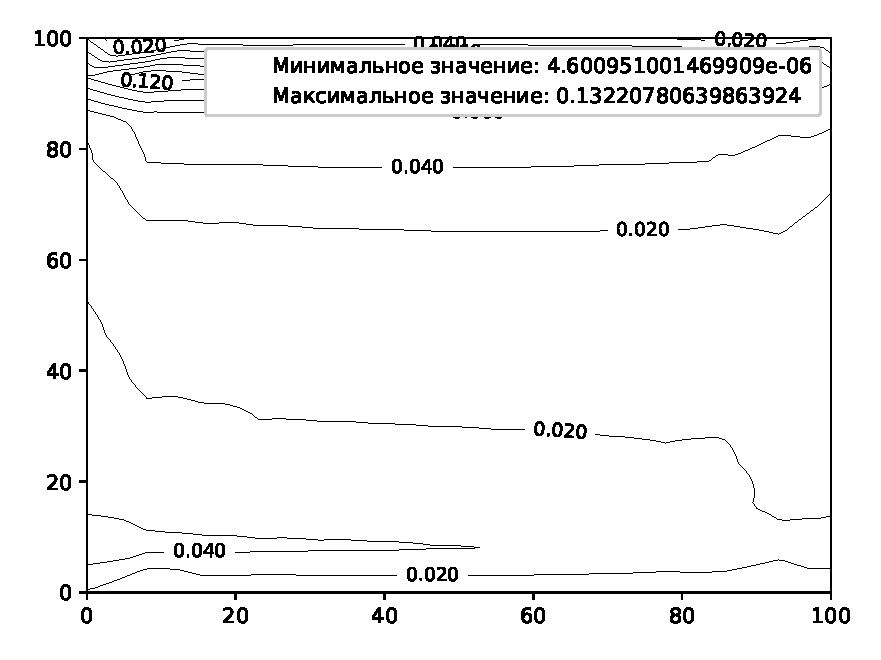
\includegraphics[width=.49\linewidth]{img/exp12/theta_n_diff_iso}
        }
        \subfloat[Изменение функционала в зависимости от числа итераций]
        { \includegraphics[width=.49\linewidth]{img/exp12/quality} }
        \caption{Результаты первого эксперимента}
    \end{figure}
    \begin{figure}[H]
        \centering
        \subfloat[$|q_n - \partial_n\theta_\lambda|$]
        { \label{fig:img_test_12_cube} 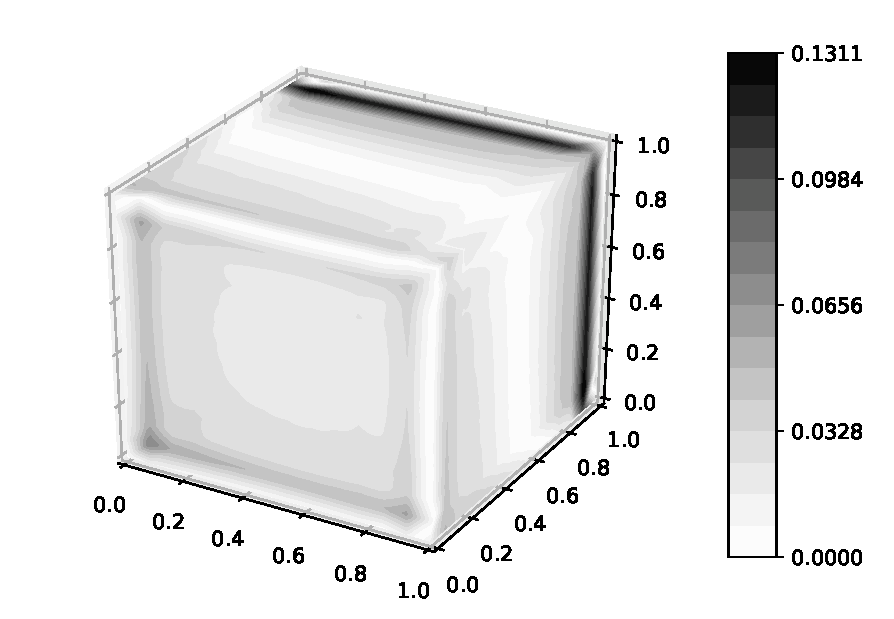
\includegraphics[width=.49\linewidth]{img/exp12/theta_n_diff_cube}
        }
        \subfloat[Изменение функционала в зависимости от числа итераций]
        { \includegraphics[width=.49\linewidth]{img/exp12/quality} }
        \caption{Результаты первого эксперимента}
    \end{figure}

    \textbf{Пример 2.}
    Сравним работу предложенного алгоритма с результатами статьи~\cite{CNSNS19}, где
    соавтором был один из авторов данной работы.
    Задача рассматривается в области $\Omega\times (-L,L)$, где $\Omega = \{ x = (x_1,x_2) \colon 0 < x_{1,2} < d\}$
    и при больших $L$ сводится к двумерной задаче с вычислительной областью $\Omega$.
    Выбраны следующие значения параметров задачи: $d = \mathrm{1(m)}$, $a = 0.92~10^{-4}~\mathrm{(m^2/s)}$, $b=
    0.19~\mathrm{(m/s)}$, $\alpha = 0.0333~\mathrm{(m)}$ и $\kappa_a = 1~\mathrm{(m^{-1})}$.
    Параметры соответствуют воздуху при нормальном атмосферном давлении и температуре 400$^\circ$C\@.

    Функции $\theta_b$, $q_b$ в краевом условии~\eqref{bc2} заданы следующим образом:
    $\theta_b = \widehat{\theta}|_{\Gamma}$, $q_b = \partial_n \widehat{\theta}|_{\Gamma}$, где
    $\widehat{\theta} = (x_1-0.5)^2 - 0.5x_2+0.75$.

    Приближенное решение задачи с данными Коши, представленное в~\cite{CNSNS19} (рис.~\ref{fig2:CNSNS19}),
    получено путем решения эллиптической задачи четвертого
    порядка для температуры методом установления по времени.
    Использовались $H^2$ конформные конечные элементы Богнера-Фокса-Шмитта и
    солвер FeliCs, разработанный в техническом университете Мюнхена.
    Решение стабилизировалось через 120 секунд, но вычисления на каждом временном
    шаге потребовали довольно значительных затрат~\cite{CNSNS19}.

    На рис.~\ref{fig2:theta_auto} представлено температурное поле, полученное
    предложенным в данной статье методом, достаточно точно совпадающее с результатом в~\cite{CNSNS19}.
    Величина $\|\partial_n\theta_\lambda-q_b\|_{L^2(\Gamma)}/\|q_b\|_{L^2(\Gamma)}$ равна $~0.000567$.
    Значение функционала качества, определяющего норму разности $\|\theta_\lambda -\theta_b\|^2_\Gamma$,
    равно $~0.000255$ и стабилизируется после 10 итераций.

    \begin{figure}[H]
        \label{fig:fig2}
        \centering
        \subfloat[Температурное поле на $\Gamma$]
        {
        \label{fig2:theta_b}
        \includegraphics[width=.49\linewidth]{img/exp2/theta_b}
        }
        \subfloat[Производная по нормали]
        {
        \label{fig2:theta_n}
        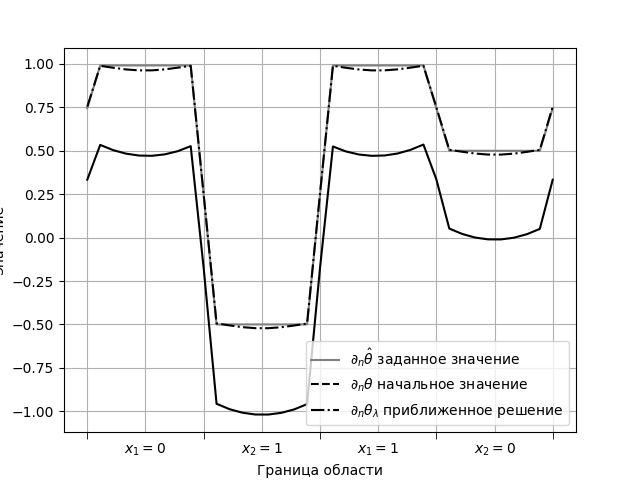
\includegraphics[width=.49\linewidth]{img/exp2/theta_n}
        }
        \caption{Графики температурного поля $\theta$}
    \end{figure}

    \begin{figure}[H]
        \centering
        \subfloat[Полученное решение $\theta$]
        {
        \label{fig2:theta_auto}
        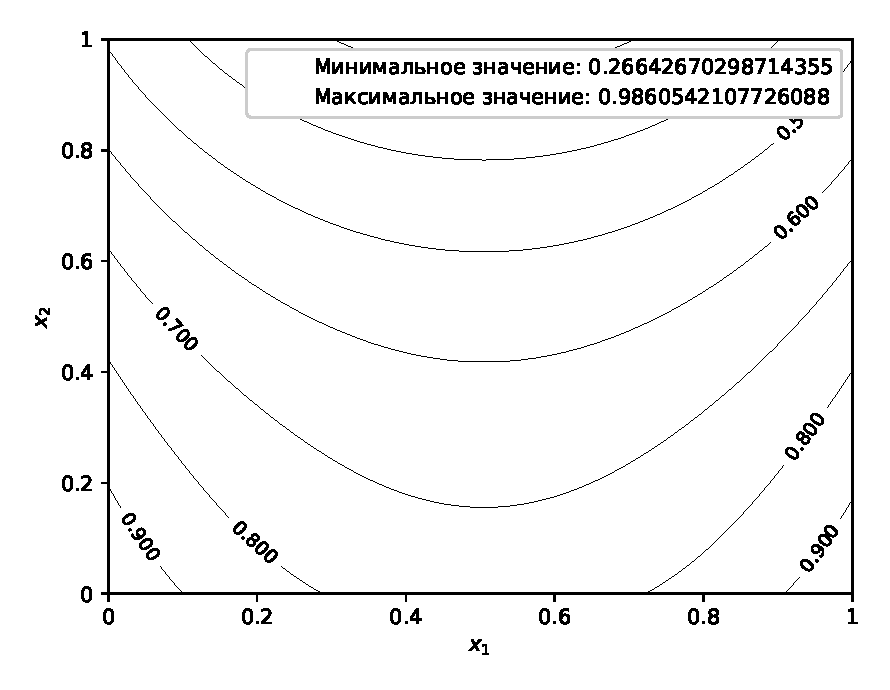
\includegraphics[width=.49\linewidth]{img/exp2/theta_auto}
        }
        \subfloat[Изменение функционала качества]
        {
        \label{fig3:quality}
        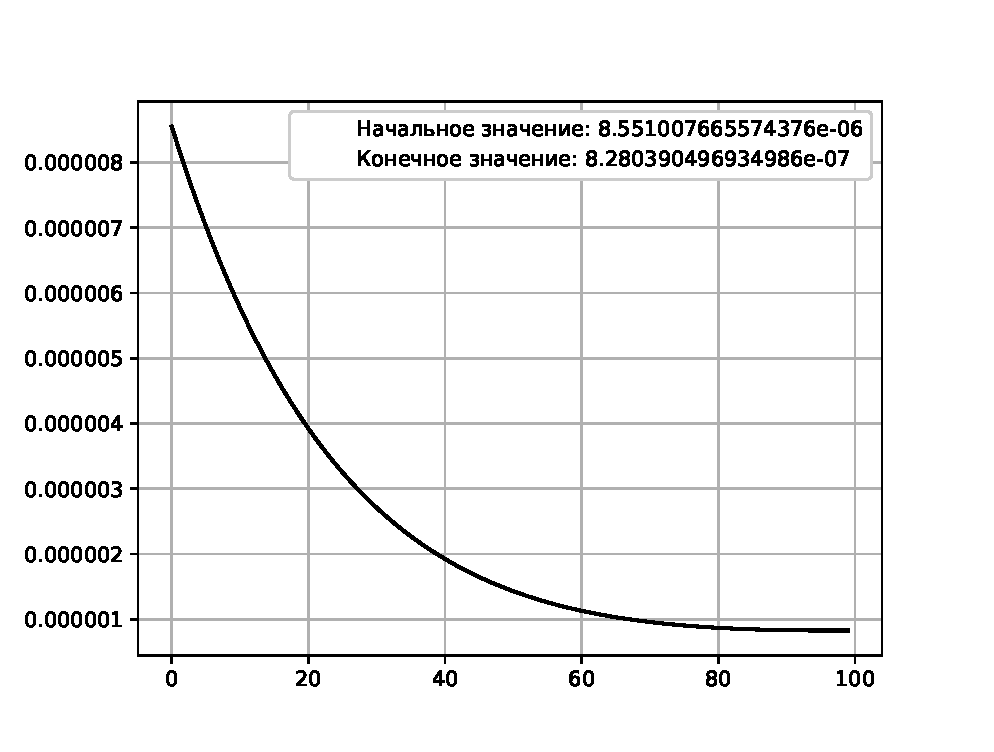
\includegraphics[width=.49\linewidth]{img/exp2/quality}
        }
        \caption{}
        \label{fig3}
    \end{figure}

    Представленные численные примеры иллюстрируют, что предложенный алгоритм успешно справляется
    с нахождением численного решения задачи~\eqref{eq1}-\eqref{bc2}.

    Исходный программный код экспериментов можно найти по ссылке~\cite{mesenev-github}.

    \begin{thebibliography}{999}

        \bibitem{Modest}
        Modest~M.F. Radiative Heat Transfer.
        Academic Press. 2003. 822 p.

        \bibitem{Kovt}
        Kovtanyuk A.E., Chebotarev A.Yu., Botkin N.D. Unique solvability of a steady-state complex heat
        transfer model // Commun. Nonlinear Sci. Numer.
        Simul. 2015. V.~20. N 3. P. 776--784.

        \bibitem{Pinnau07}
        R.~Pinnau. Analysis of Optimal Boundary Control for Radiative Heat
        Transfer Modelled by the SP$_1$-System~// Comm.
        Math. Sci. 2007. V.~5. N~4. P.~951--969.

        \bibitem{Tse12}
        Tse O., Pinnau R., Siedow N. Identification of temperature
        dependent parameters in laser--interstitial thermo therapy~//
        Math. Models Methods Appl. Sci. 2012. V.~22. N~9. P. 1--29.

        \bibitem{Kovt13}
        Kovtanyuk~A.E., Chebotarev~A.Yu. An iterative method for solving a
        complex heat transfer problem~// Appl.
        Math. Comput. 2013. V.~219. P.~9356--9362.

        \bibitem{Cheb14-1}
        Kovtanyuk~A.E., Chebotarev~A.Yu., Botkin~N.D., Hoffmann~K.-H. The
        unique solvability of a complex 3D heat transfer problem~// J.
        Math. Anal. Appl. 2014. V.~409. N~2. P.~808-815.

        \bibitem{JVM-14}
        Ковтанюк А.Е., Чеботарев А.Ю. Стационарная задача сложного теплообмена // Ж.
        вычисл. матем. и матем. физ. 2014. Т. 54. \textnumero~4. С. 711--719.

        \bibitem{Kovt14-2}
        Ковтанюк А.Е., Чеботарев А.Ю. Стационарная задача свободной конвекции с радиационным теплообменом // Дифференц.
        ур-ния. 2014. Т. 50. \textnumero~12. С. 1590--1597.

        \bibitem{Kovt14-3}
        Kovtanyuk A.E., Chebotarev A.Yu., Botkin N.D., Hoffmann K.-H. Theoretical analysis of an optimal
        control problem of conductive-convective-radiative heat transfer // J. Math.
        Anal. Appl. 2014. V. 412. \textnumero~1. P. 520--528.

        \bibitem{Grenkin1}
        Гренкин Г.В., Чеботарев А.Ю. Нестационарная задача сложного теплообмена // Ж.
        вычисл. матем. и матем. физ. 2014. Т. 54. \textnumero~11. С. 1806--1816.

        \bibitem{Grenkin3}
        Гренкин Г.В., Чеботарев А.Ю. Неоднородная нестационарная задача сложного теплообмена // Сиб.
        электрон. матем. изв. 2015. Т. 12. С. 562--576.

        \bibitem{Grenkin4}
        Гренкин Г.В., Чеботарев А.Ю. Нестационарная задача свободной конвекции с радиационным теплообменом // Ж.
        вычисл. матем. и матем. физ. 2016. Т. 56. \textnumero~2. С. 275--282.

        \bibitem{Grenkin5}
        Grenkin G.V., Chebotarev A.Yu., Kovtanyuk A.E., Botkin N.D., Hoffmann K.-H. Boundary optimal control problem
        of complex heat transfer model // J. Math.
        Anal. Appl. 2016. V. 433. \textnumero~2. P. 1243--1260.

        \bibitem{JMAA-16}
        Kovtanyuk A.E., Chebotarev A.Yu., Botkin N.D., Hoffmann K.-H. Optimal boundary control of a steady-state heat
        transfer model accounting for radiative effects // J. Math.
        Anal. Appl. 2016. V. 439. \textnumero~2. P. 678--689.

        \bibitem{AMC-16}
        Chebotarev A.Yu., Kovtanyuk A.E., Grenkin G.V., Botkin N.D., Hoffmann K.-H.
        Nondegeneracy of optimality conditions in control problems for a radiative-conductive heat transfer model
        // Appl.
        Math. Comput. 2016. V. 289. P. 371--380.

        \bibitem{JVM-16}
        Ковтанюк А.Е., Чеботарев А.Ю. Нелокальная однозначная разрешимость стационарной задачи сложного теплообмена
        // Ж.
        вычисл. матем. и матем. физ. 2016. Т. 56. \textnumero~5. С. 816--823.

        \bibitem{ESAIM}
        Chebotarev A.Yu., Grenkin G.V., Kovtanyuk A.E. Inhomogeneous steady-state problem of complex heat transfer //
        ESAIM Math.
        Model. Numer. Anal. 2017. V. 51. \textnumero~6. P. 2511--2519.

        \bibitem{JMAA-18}
        Chebotarev A.Yu., Grenkin G.V., Kovtanyuk A.E., Botkin N.D., Hoffmann K.-H. Inverse problem with finite
        overdetermination for steady-state equations of radiative heat exchange // J. Math.
        Anal. Appl. 2018. V. 460. \textnumero~2. P. 737--744.

        \bibitem{JMAA-19}
        Chebotarev A.Yu., Pinnau R. An inverse problem for a quasi-static approximate model of radiative heat transfer
        // J. Math.
        Anal. Appl. 2019. V. 472. \textnumero~1. P. 737--744.


        \bibitem{AmosA05}
        Амосов~А.А. Глобальная разрешимость одной нелинейной
        нестационарной задачи с нелокальным краевым условием типа
        теплообмена излучением~// Дифференц.
        ур-ния. Т.~41. N~1. 2005. С.~93--104.

        \bibitem{AmosA10}
        Amosov~A.A. Stationary nonlinear nonlocal problem of
        radiative-conductive heat transfer in a system of opaque bodies
        with properties depending on the radiation frequency~// J.
        Math. Sc. 2010. V.~164. N~3. P.~309--344.

        \bibitem{Amosov16}
        Amosov A. Unique Solvability of a Nonstationary Problem of Radiative - Conductive
        Heat Exchange in a System of Semitransparent Bodies // Russian J. of Math.
        Phys. 2016. V. 23, N~3. P.~309-334.

        \bibitem{Amosov17}
        Амосов А.А. Стационарная задача сложного теплообмена в системе полупрозрачных тел с краевыми условиями
        диффузного отражения и преломления излучения // Ж.
        вычисл. матем. и матем. физ. 2017. Т. 57. \textnumero~3. С. 510--535.

        \bibitem{Amosov17-1}
        Amosov A.A. Unique Solvability of Stationary Radiative - Conductive Heat Transfer
        Problem in a System of Semitransparent Bodies // J. of Math.
        Sc.(United States). 2017. V. 224. N~5. P.~618-646.

        \bibitem{Amosov18}
        Amosov A.A. Nonstationary problem of complex heat transfer in a system of
        semitransparent bodies with boundary-value conditions of diffuse reflection and refraction
        of radiation // J. of Math. Sc.(United States). 2018. V. 233. N~6. P.~777 -806.

        \bibitem{CNSNS19}
        Chebotarev A.Yu., Kovtanyuk A.E., Botkin N.D. Problem of radiation heat exchange with boundary conditions
        of the Cauchy type // Commun.
        Nonlinear Sci. Numer. Simul. 75 (2019) 262-269.

        \bibitem{CMMP20}
        Колобов А.Г., Пак Т.В., Чеботарев А.Ю. Стационарная задача радиационного теплообмена с граничными условиями
        типа Коши // Журнал вычислительной математики и математической физики.
        2019, том 59, № 7, с. 1258-1263.


        \bibitem{Kufner} S.~Fu\v{c}ik, A.~Kufner, Nonlinear differential equations,
        Elsevier, Amsterdam--Oxford--New York, 1980.

        \bibitem{10} A.V.~Fursikov, Optimal Control of Distributed
        Systems. Theory and Applications, American Math. Soc., 2000.

        \bibitem{11} A.D.~Ioffe, V.M.~Tikhomirov, Theory of Extremal
        Problems, North-Holland, Amsterdam, 1979.

    \end{thebibliography}


\end{document}
